\documentclass{article}

\usepackage{neurips_2026}

\usepackage[utf8]{inputenc}
\usepackage[T1]{fontenc}
\usepackage{hyperref}
\usepackage{url}
\usepackage{booktabs}
\usepackage{amsfonts}
\usepackage{amsmath}
\usepackage{amssymb}
\usepackage{nicefrac}
\usepackage{microtype}
\usepackage{xcolor}
\usepackage{graphicx}

\title{Rule-Conditioned Neural Cellular Automata as World Models for
PuzzleScript Games}

\author{%
  Anonymous \\
  Affiliation \\
  \texttt{anonymous@example.com} \\
}

\begin{document}

\maketitle

\begin{abstract}
We study learned world models for the PuzzleScript family of grid-based
puzzle games---a domain with sharply combinatorial dynamics, deterministic
discrete states, hand-authored rule sets that often induce iterative
\texttt{again} loops, and dozens of distinct games sharing a common
substrate. We propose a \emph{rule-conditioned Neural Cellular Automaton}
(NCA) world model in which a perceiver-style encoder maps each game's
tokenized rule set to $K$ slot vectors, and a shared local update rule
applied for $T$ iterations cross-attends to those slots at every step.
This architecture mirrors the engine's own two-level loop
(an ordered list of rules applied repeatedly until convergence) and
generalizes across games at modest scale. We benchmark this model
against three non-NCA baselines that share the slot encoder but replace
the iterated local update with a non-iterative spatial body: a deep
ResNet, a U-Net, and a ViT with global self-attention. The comparison
isolates the contribution of the iterated-local-update inductive bias
from the conditioner. We additionally study adaptive halting via
PonderNet- and convergence-style stopping rules, and characterize a
ceiling that arises in the multi-grid synthetic-data regime where the
model can no longer memorize per-state outcomes. We release tooling
that packages the comparison reproducibly across a fourteen-game
benchmark.
\end{abstract}

\section{Introduction}
\label{sec:intro}

Learned world models have been studied primarily in settings where
the environment is observed as pixels and the task is to predict the
next frame or latent video token. The standard recipe pairs a
high-capacity visual encoder--decoder---typically a CNN, U-Net, or
video Transformer---with an action-conditioned dynamics module. This
is a natural fit when the observation is visually rich and the
underlying mechanics are comparatively smooth or uniform. It is a
less natural fit for games whose difficulty lies not in rendering but
in a large space of symbolic rule systems.

PuzzleScript games are such a regime. Each game is fully specified by
a short text file describing object kinds, layered grid levels, and a
list of declarative rewrite rules, e.g.
\texttt{[ > Player | Crate ] -> [ > Player | > Crate ]}. The engine
evaluates these rules in order on the grid at every tick, applying each rule until the state converges, with \texttt{again} rules causing the entire rule block to fire again. The state can be represented as a discrete multi-channel
grid, the dynamics are deterministic and combinatorial, and
the hard computation per tick is a sequence of atomic local updates
applied repeatedly.

To capture this symbolic mechanical complexity, we propose a \emph{rule-conditioned Neural
Cellular Automaton} (NCA) world model.
A perceiver-style encoder maps
the tokenized game description to $K$ latent slots; the dynamics body
is a local update rule applied for $T$ iterations on a hidden grid,
with cells cross-attending to those slots at every step. The same body
parameters can be reused across iterations, mirroring the engine's
outer loop, while the conditioner makes the dynamics model portable
across games. In the full version of the model, these slots are tied
to a symbolic-game autoencoder so that game latents can both condition
dynamics and decode back into program text.
Foregoing pixels lets us model the environment in
its native state representation and measure fidelity cell-by-cell
against the original engine.

Our corpus contains 3{,}474 token-distinct
human-authored games (one to twenty rules each), of which up to 199
are used in the largest training preset. Across these games we cache
bounded-A* transitions from authored levels, yielding $\sim$15M
transitions; held-out evaluation uses a 30-game stratified sample
disjoint from training by name and token-sequence hash.

On the 94-game broad-corpus training preset, the trained NCA achieves
a median per-cell teacher-forced one-step error of $0.15\%$ and a
median 50-step random-action autoregressive rollout error of
$2.5\%$ across all 94 games and all authored levels.
% We use ``near-perfect'' to mean a one-step teacher-forced cell-error rate below $1\%$ on the broad corpus, with the multi-step rollout numbers quantifying the drift caused by autoregressive compounding.
To rule out per-state memorization, we also report a
within-game OOD-levels probe (\S\ref{sec:results-within-game}) in
which every authored level is held out from training and only
purely-synthetic rollouts at the same grid size enter the training
set; the same rule-conditioned NCA recovers near-zero rollout error
on all authored levels of Sokoban-class games and non-trivial
transfer on three further mechanic classes, evidencing that the
high-precision regime reflects learned rule structure rather than
authored-state lookup.

\paragraph{Contributions.}
\begin{enumerate}
  \item \textbf{NCA dynamics over discrete state.}
        Modeling the engine's native discrete grid with a shared,
        iteratively-applied local update body matches the reference
        dynamics with median 1-step teacher-forced cell-error of
        $0.15\%$ across the 94-game broad-corpus preset. A controlled
        comparison that holds the rule encoder fixed and varies only
        the spatial body shows the iterated-local-update bias
        outperforms non-iterative architectures (CNN, U-Net, ViT) on
        rollout fidelity at matched or smaller parameter counts.
        Within-game OOD-levels probes (\S\ref{sec:results-within-game})
        confirm the model is learning rule structure rather than
        memorizing authored states.
  \item \textbf{Rule-conditioning for multi-game simulation.}
        A single model simulates dozens of mechanically diverse games
        by cross-attending to slot embeddings produced by an encoder
        over each game's tokenized rule text. Trained jointly with a
        slot-token decoder, the same latent drives forward dynamics
        and decodes back to program text: $76/94$ training games
        reconstruct perfectly under teacher forcing, $15/25$ samples
        from the empirical slot prior decode to engine-loadable
        PuzzleScript, and slot-space interpolation between two games
        is engine-loadable at $9/9$ points along the line.
        The same latent is also recoverable by inverse-fitting through
        the frozen NCA, driving per-cell BCE 2--3 orders of magnitude
        down on held-out targets and snapping the optimised slot to
        mechanically-related training games.
  \item \textbf{Generalization to unseen games.}
        On a 30-game held-out set disjoint from training by name and
        token-sequence hash, we evaluate two axes of engine-level
        transfer: \emph{geometric} placement of held-out latents
        relative to training-game latents, and \emph{predictive}
        accuracy of the dynamics model on novel rule combinations.
        The results delineate where the rule-conditioned NCA
        generalizes today and where further work is needed.
\end{enumerate}

\section{Related Work}
\label{sec:related}

\paragraph{Neural Cellular Automata.}
Neural Cellular Automata learn a local update rule that, applied
repeatedly to a grid of hidden states, gives rise to globally
coordinated behavior~\cite{mordvintsev2020growing}. Subsequent work has
demonstrated NCAs that grow morphologies from a seed, classify under
distribution shift, perform texture synthesis, and self-organize
attention~\cite{niklasson2021selforganising,palm2022variational,najarro2022hypernca}.
NCAs are typically trained with stochastic update schedules and a
``pool'' of intermediate states for stability. Recent work treats the
NCA's iteration count as a meaningful axis of computation and studies
when more iterations buy more reasoning. Our use of NCAs as
\emph{action-conditioned world models} extends this line: rather than
asking the NCA to converge to a static target, we ask it to predict
the engine's deterministic next state at every tick.

\paragraph{World models and self-prediction.}
World-model literature dates back at least to Schmidhuber's curiosity
work and was popularized for vision-based RL by
Ha and Schmidhuber~\cite{ha2018world}. Recent transformer-based
world models~\cite{micheli2022iris,robine2023transformer} compress
images to discrete tokens and roll out dynamics autoregressively over
those tokens; PWM-style methods integrate planning into a learned
model. Our problem domain---fully discrete grid observations,
authored rule sets, dozens of related games sharing a substrate---is
closer to procedural-content benchmarks like NetHack and CHAI than to
Atari. Compared to MuZero-style models that learn an abstract latent
dynamics, our model commits to predicting the engine's next state in
its native grid representation, which makes ground-truth supervision
exact and lets us compare to the engine cell-by-cell.

\paragraph{PuzzleScript and rule-based puzzle games.}
PuzzleScript~\cite{lavelle2013puzzlescript} is a domain-specific
language for grid-based puzzle games that supports a rich family of
authoring patterns: chained pushing (\texttt{[ Crate | Crate ] -> [
Crate | Crate ]}), \texttt{again}-driven simulation (gravity, ball
trajectories, light beams), multi-character control, and rule
priorities. Several hundred community games are publicly available and
share both a tokenization scheme (the engine source) and a common
state encoding, making the family a natural multi-game benchmark for
world models. Prior work has studied PuzzleScript primarily for
procedural content generation and human play; to our knowledge, ours
is the first systematic study of learned forward models on a broad
PuzzleScript gallery.

\paragraph{Adaptive computation.}
PonderNet~\cite{banino2021pondernet} learns a per-input halting
distribution over a recurrent module, with a KL prior over the number
of iterations. Adaptive Computation Time~\cite{graves2016act} and
Universal Transformers~\cite{dehghani2018universal} are predecessors.
Our adaptive-halt experiments adapt PonderNet to NCA world models
with a shared body, so that ``halt at step $k$'' coherently asks the
same rule set to converge in $k$ iterations rather than selecting
between $k$ different models.

\paragraph{Learned local-update grids more broadly.}
ConvLSTMs~\cite{shi2015convlstm}, graph neural networks, and
diffusion-style iterative refinement all share with NCAs the high-level
idea of repeated local computation. NCAs differ in committing to a
\emph{shared} (across iterations) update rule on a fixed grid, which
matches the PuzzleScript engine's outer-loop semantics. A detailed
comparison to procedural / engine-aligned NCA work is deferred to
the appendix.

\section{Method}
\label{sec:method}

\subsection{Problem setup}

A PuzzleScript game is a tuple $(\mathcal{O}, R, \{L_i\})$ where
$\mathcal{O}$ is an ordered list of object kinds, $R$ is a list of
rewrite rules, and $\{L_i\}$ are authored levels. Each level is a
multi-channel grid $s \in \{0,1\}^{C \times H \times W}$ where channel
$c$ is the indicator of object kind $c$ at each cell. An action $a \in
\{\texttt{up}, \texttt{down}, \texttt{left}, \texttt{right},
\texttt{action}\}$ together with the current state $s_t$
deterministically yields a next state $s_{t+1}$ via the engine. The
state can also carry a terminal \emph{won} bit, since some rules
trigger a win on certain conditions.

We train a model $f_\theta(s_t, a_t, \mathrm{spec}) \mapsto
\widehat{s}_{t+1}$ where $\mathrm{spec}$ is the tokenized game source
(a sequence of integers from a shared $\sim$140-symbol vocabulary that
covers the engine's grammar plus per-game object names and 5$\times$5
sprite RGBA values when sprite tokens are enabled). At evaluation we
roll the model out autoregressively and compare cell-by-cell against
the engine.

\subsection{Rule-conditioned NCA world model}

\paragraph{Slot encoder.}
A perceiver-style encoder $\mathrm{Enc}_\phi$ maps the game's token
sequence $\mathrm{spec} \in \mathbb{Z}^{S}$ to $K$ slot vectors $z \in
\mathbb{R}^{K \times d}$. The encoder applies $\ell$ self-attention
layers over the tokens, then $K$ learned query vectors cross-attend
into the contextualized token sequence to produce $z$. Slots are
shared across cells and remain fixed throughout the rollout.

\paragraph{NCA dynamics body.}
We embed the input $(s_t, a_t)$ into a hidden grid $h^{(0)} \in
\mathbb{R}^{H \times W \times d_h}$ via a single dense layer applied
to the per-cell concatenation of $s_t$'s channels and a broadcast
one-hot action. We then apply $T$ NCA steps:
\begin{align}
  h^{(k+1)} &= h^{(k)} + W_o \,\mathrm{GELU}\!\bigl(
      W_c\, [\, h^{(k)} \,;\, h^{(0)} \,]_{3\times 3}
      \;+\;
      \mathrm{XAttn}(h^{(k)}, z)
    \bigr) \, ,
\end{align}
where $[\,\cdot\,]_{3\times 3}$ denotes a $3{\times}3$ convolution
producing a vector at each cell, $\mathrm{XAttn}$ is a multi-head
attention with each cell as a query and the $K$ slots as keys/values,
and $W_o, W_c$ are shared across all $T$ steps. The
\emph{input-skip} concatenation re-injects the embedded
$(s_t, a_t)$ at every step, preventing the deep unroll from drifting.

\paragraph{Pool features.}
A bare $3{\times}3$ convolution can only propagate one cell of context
per NCA step, but several PuzzleScript rule patterns reference cells
that are arbitrarily far apart (\texttt{[ X | ... | Y ]} along an
axis, or \texttt{[X][Y]} anywhere in the grid). We therefore augment
each step with three optional pool feature stacks:
axis max pool (row-max and col-max), axis cumulative max
(directional prefix-max in each of four directions), and global max
pool. These features are computed from the current hidden grid and
broadcast back to every cell before the convolution, exposing
non-local information that would otherwise require $\Omega(\max(H,W))$
NCA steps to surface.

\paragraph{Hierarchical weight sharing.}
Inspired by the engine's two natural levels of iteration (an inner
ordered list of rules + an outer \texttt{again} re-evaluation loop),
we factor $T = n_\ell \cdot n_r$ where $n_\ell$ distinct layers form
the inner block and $n_r$ outer applications share weights. Setting
$n_r = T$ recovers a single shared layer applied $T$ times (matches
the engine's outer-loop structure); setting $n_r = 1$ recovers the
usual per-step body with $T$ distinct layers.

\paragraph{Heads.}
A shared \texttt{readout} dense layer maps the final $h^{(T)}$
cell-wise to next-state logits $\widehat{s}_{t+1} \in \mathbb{R}^{C
\times H \times W}$; a separate dense layer over the spatially
average-pooled $h^{(T)}$ produces a binary win logit. Training loss
is a per-cell BCE on the next-state with an upweight on cells that
\emph{change} between $s_t$ and $s_{t+1}$, plus a binary cross-entropy
on the win head.

\subsection{Baselines}

We compare against three non-NCA baselines that share the slot
encoder $\mathrm{Enc}_\phi$, the input embedding, and the readout
heads, but replace the NCA body. Each baseline consumes
$h^{(0)}$ and the slots $z$ and emits a final hidden grid $h^{(T)}$
of the same shape; the comparison isolates the contribution of the
spatial-update body.

\begin{itemize}
  \item \textbf{CNN}: a stack of $n_b$ residual blocks, each
    containing the same conv + optional pool + slot-cross-attn +
    residual gate as one NCA layer, but with \emph{distinct}
    weights per block and applied once. Tests whether iteration with
    weight sharing matters at all.
  \item \textbf{U-Net}: a 2-level encoder--decoder with skip
    connections and a FiLM bottleneck that reads pooled slots. Tests
    whether multi-scale hierarchy substitutes for repeated local
    updates.
  \item \textbf{ViT}: $n_v$ Transformer encoder layers over the
    flattened cell sequence with learned 2D positional embedding,
    plus a slot cross-attention and feed-forward block per layer.
    Tests whether unrestricted global attention beats locality plus
    iteration.
\end{itemize}

All baselines accept the same input $(s_t, a_t, \mathrm{spec})$ and
produce the same $(\widehat{s}_{t+1}, \widehat{w}_{t+1})$ outputs as
the NCA, allowing identical training and evaluation pipelines.

\subsection{Adaptive halting (optional)}
\label{sec:method-halt}

A fixed $T$ is wasteful for easy transitions and insufficient for
hard ones. We add an optional halting head: at each NCA step $k$, a
small dense layer reads the spatially pooled $h^{(k)}$ and emits a
halt logit $\lambda_k$. The induced halt distribution
$p_k = \mathrm{sigmoid}(\lambda_k) \prod_{j<k}(1 - \mathrm{sigmoid}(\lambda_j))$
weights the per-step loss
$\mathcal{L}_{\text{rec}} = \sum_k p_k \mathcal{L}_k$
plus a KL-to-geometric-prior regularizer
$\mathrm{KL}(p \,\|\, \mathrm{Geom}(p_0))$. We additionally study a
\emph{convergence-stopping} baseline that halts at inference when
consecutive predictions stop changing, with no learned halt head.

\section{Experimental setup}
\label{sec:experiments}

\subsection{Data}

We collect $(s_t, a_t, s_{t+1}, w_{t+1})$ transitions for each game by
running the C++ PuzzleScript engine under bounded A* search from each
authored level. Each transition is cached on disk (bit-packed for
roughly 8$\times$ compression) and re-used across runs. For
multi-game training we draw batches with one share per game per step
(\emph{balanced sampling}), which compensates for per-game dataset-size
imbalance.

\paragraph{Synthetic levels.}
For ablations and held-out evaluations we additionally generate
synthetic levels by sampling tile-pattern distributions from each
game's authored levels and validating each candidate by running the
engine to confirm the level is solvable and exposes a non-trivial
state space (more details in the appendix). The validated synthetic
recipe (per-game sizes, fallback dynamics, multi-grid widths) is what
allowed our model to match the authored-data baseline on the
\textsc{nekopuzzle} game without overfitting to grid-size artifacts.

\subsection{Game suites}

We evaluate on three suites of increasing breadth:

\begin{itemize}
  \item \textbf{Single-game} (\textsc{microban}, 10 authored levels):
    classic chained Sokoban pushing on small grids. Used for
    architecture ablations where dynamics complexity is fully
    controlled.
  \item \textbf{Single-game / synthetic-multi-grid}
    (\textsc{sokoban\_basic}): a controlled stress test in which the
    model is trained on synthetic levels of multiple grid sizes
    $\{5{\times}5, 6{\times}6, 7{\times}7, 8{\times}8\}$ and evaluated
    on the same. The diversity prevents per-state memorization and
    forces the model to learn the underlying rule.
  \item \textbf{Multi-game} (\textsc{scaling\_14}): a fourteen-game
    benchmark including chained pushing, gravity, light beams,
    multi-character control, and several \texttt{again}-driven
    simulations. Per-game grid sizes range from $4{\times}4$ to
    $32{\times}24$.
\end{itemize}

\subsection{Architectures and hyper-parameters}

All models share the same input embedding (Dense over
$(s_t \,\|\, \mathrm{onehot}(a_t))$) and readout heads. The slot
encoder is identical across architectures: $K{=}16$ slots, $d{=}64$
slot dim, two self-attention layers over tokens, four heads.

The NCA uses $T{=}4$ NCA steps with $n_r{=}T$ (single shared layer
applied $T$ times), $d_h{=}256$, full pool features, input-skip on,
optional padding mask for multi-grid. The CNN baseline uses
$n_b{=}4$ residual blocks; the U-Net uses 2 levels of down/up
sampling with bottleneck FiLM; the ViT uses $n_v{=}4$ layers, four
heads. We report parameter count alongside every metric so the
comparison is honest.

Training: Adam, learning rate $3 \times 10^{-4}$ with cosine decay
to $10^{-7}$, gradient clipping at global norm $0.5$, batch size 32,
\emph{change-loss-weight} $5.0$ (per-cell BCE upweighted on cells
that change between $t$ and $t+1$), and patience-based early stop on
the change-accuracy metric. Each run is replicated with three random
seeds.

\subsection{Evaluation}

We report two complementary metrics:
\begin{itemize}
  \item \textbf{One-step change-error}: the per-cell BCE-thresholded
    error rate on the cells that change between $s_t$ and $s_{t+1}$,
    measured under teacher forcing on the held-out portion of each
    cache.
  \item \textbf{Autoregressive rollout error}: the same per-cell error
    averaged over a 50-step rollout from each level's start state,
    under three policies: random actions, BFS-optimal, and A*-optimal.
\end{itemize}
Per finding F3 in our architecture report~(\S\ref{sec:results}), train
loss decouples from autoregressive rollout error in the
over-capacity regime; reporting both is essential.

\section{Results}
\label{sec:results}

\subsection{Baselines vs.\ rule-conditioned NCA}
\label{sec:results-baselines}

Table~\ref{tab:baselines-microban} reports the head-to-head comparison
on \textsc{microban} (10 authored levels), trained for 10k updates per
seed at $d_h = 256$ with the canonical recipe (\S\ref{sec:experiments}).
We measure best train cross-entropy loss, end-of-rollout cell-error
rate under three policies (random, BFS-optimal, A*-optimal), and final
parameter count. The table reports a single seed; the multi-seed
synthetic-data comparison is reported in
Table~\ref{tab:baselines-synth}.

\begin{table}[t]
  \centering
  \caption{\textbf{Baselines vs.\ rule-conditioned NCA on
    \textsc{microban} (authored levels).} Single seed at 10k updates.
    Lower is better for loss and cell-error; A* first-divergence step
    is higher-is-better. Param count is in millions.}
  \label{tab:baselines-microban}
  \small
  \begin{tabular}{l c c c c c}
    \toprule
    Architecture & params (M) & best loss & BFS final-err & rand mean-err & A* first-div \\
    \midrule
    \textbf{NCA (shared, $T{=}4, n_r{=}T$)} & \textbf{1.94} & 0.106 & 0.34\% & 0.04\% & 64 \\
    NCA (per-step, $T{=}4, n_r{=}1$)        & 7.36          & 0.107 & 0.00\% & 0.09\% & none \\
    CNN (4-block ResNet)                    & 5.00          & 0.107 & 0.00\% & 0.09\% & none \\
    U-Net (2 levels)                        & 6.07          & 0.107 & 6.27\% & 3.00\% & 12 \\
    ViT (4 layers)                          & 3.99          & 0.107 & 11.67\% & 6.07\% & 1 \\
    \bottomrule
  \end{tabular}
\end{table}

Three findings on this controlled, memorizable single-game setting:
\textbf{(i)} the NCA with shared weights matches CNN / per-step NCA
on oracle-policy rollout error at $2.5{-}3.8\times$ fewer parameters,
\textbf{(ii)} U-Net and ViT both actively underperform despite
parameter counts comparable to or exceeding NCA-shared --- U-Net's
2-level downsampling loses fine-grained player position on small
grids, and ViT's global self-attention diverges within the first
rollout step (mean first-divergence step $0.8$), suggesting
locality plus iteration is a stronger inductive bias for grid-rule
dynamics than unrestricted global attention; and \textbf{(iii)} best
train loss is essentially identical (0.106--0.107) across all five
architectures, illustrating finding F3 (\S\ref{sec:results-F3}):
train loss is invisible to a $\geq 30\times$ swing in autoregressive
rollout error (0.34\% vs.\ 11.67\%).

\medskip\noindent
The full comparison on the multi-grid synthetic data
regime---where memorization is unavailable and rule learning is
required---is reported in Table~\ref{tab:baselines-synth} and
analyzed in \S\ref{sec:results-ceiling}.

\begin{table}[t]
  \centering
  \caption{\textbf{Baselines vs.\ rule-conditioned NCA on
    \textsc{sokoban\_basic} (multi-grid synthetic).} Single seed at 10k
    updates; widths $\{5{\times}5, 6{\times}6, 7{\times}7, 8{\times}8\}$
    with 256 synthetic levels per width. Memorization is unavailable;
    the model has to learn the rule. Architectures sorted by BFS final
    cell-error (lower is better). Multi-seed numbers are forthcoming.}
  \label{tab:baselines-synth}
  \small
  \begin{tabular}{l c c c c}
    \toprule
    Architecture & params (M) & best loss & BFS final-err & A* final-err \\
    \midrule
    \textbf{NCA (shared, $T{=}4, n_r{=}T$)} & \textbf{3.07} & \textbf{0.067} & \textbf{3.57\%} & \textbf{3.57\%} \\
    NCA (per-step, $T{=}4, n_r{=}1$)        & 8.49          & 0.068          & 4.76\%          & 4.76\% \\
    CNN (4-block ResNet)                    & 5.00          & 0.067          & 8.33\%          & 8.33\% \\
    U-Net (2 levels)                        & 6.07          & 0.070          & 9.52\%          & 9.52\% \\
    ViT (4 layers)                          & 3.99          & 0.085          & 11.90\%         & 11.90\% \\
    \bottomrule
  \end{tabular}
\end{table}

The synthetic-multi-grid setting is the headline comparison: per-state
memorization is impossible (256 levels per width $\times$ 4 widths
$=$ 1024 distinct levels share one rule set), so the model has to
\emph{learn the slide rule}. Three observations: \textbf{(i)} the
NCA with shared weights wins on BFS rollout error (3.57\%) at the
fewest parameters (3.07M), beating the same-depth feed-forward CNN
by $2.3\times$ in error and at $1.6\times$ fewer params;
\textbf{(ii)} U-Net (9.52\%) and ViT (11.90\%) both underperform
here as well, with U-Net's hierarchical bias actively losing in this
discrete-grid regime and ViT's global attention failing to even
\emph{fit} the train loss (0.085 vs.\ 0.067 for the other four);
\textbf{(iii)} train loss now does begin to discriminate
architectures (ViT's 0.085 outlier), but NCA-shared, NCA-per-step,
and CNN are again indistinguishable on train loss (0.067--0.068)
despite a $2.3\times$ difference in BFS rollout error --- F3 still
applies.

\paragraph{(F1) Pool features are load-bearing.}
A bare $3{\times}3$ convolution can only propagate one cell of context
per NCA step. Several PuzzleScript rule patterns reference cells
arbitrarily far apart along an axis or anywhere on the level
(\texttt{[X | ... | Y]}, \texttt{[X][Y]}). Without pool features the
NCA needs $\Omega(\max(H,W))$ steps just to surface non-local
information; with axis-cummax + global pool one step suffices.
Across the 19-game \textsc{scaling\_large} preset and a controlled
\textsc{collapse} no-pool ablation, turning pool off costs both
convergence speed and final loss, with the no-pool model collapsing
into the identity-prediction minimum even at $4{\times}$ the depth.

\paragraph{(F2) Shared NCA-body weights are the right inductive bias.}
The PuzzleScript engine has two natural levels of iteration: an
inner ordered list of rules applied once each per tick, and an outer
\texttt{again} loop that re-runs the rule list until the state stops
changing. We factor $T = n_\ell \cdot n_r$ accordingly. On a single-game
depth sweep ($T \in \{2, 4, 8, 16\}$), shared $T{=}8$ reaches
$5.5{\times}$ lower train loss with $7{\times}$ fewer parameters than
the per-step body at the same depth; shared $T{=}2$ at 14$\times$
fewer parameters than the deepest per-step variant matches it on
oracle-action rollouts. Hierarchical $n_r > 1$ sits between these
extremes and is the subject of an ongoing ablation
(\S\ref{sec:results-hierarchy}).

\paragraph{(F3) Train loss decouples from autoregressive rollout error.}
\label{sec:results-F3}
A model with the lowest train (per-step) loss is not the model with
the lowest autoregressive rollout error. Concretely, in the
over-capacity regime we observe per-step models with
$5{\times}$ lower train loss but $3{-}4{\times}$ higher 50-step
rollout error. The mechanism is small but systematic per-step errors
compounding destructively under autoregression. Reporting only
best-loss hides the rollout-drift cost of going deeper or wider.

\subsection{Pool-feature ablation}
\label{sec:results-pool}

[Figure: pool-on vs.\ pool-off on \textsc{collapse}, both at depths
$T \in \{2, 4, 8, 16\}$, reporting train loss + autoregressive
rollout error.]

\subsection{Hierarchical weight sharing}
\label{sec:results-hierarchy}

[Figure: $T{=}16$ varying $n_r \in \{1, 2, 4, 8, 16\}$ on
\textsc{microban} multi-grid synth and on the multi-game
\textsc{scaling\_14} preset. Reports change-error and parameter count.]

\subsection{Adaptive halting}
\label{sec:results-halting}

We compare four halting modes and a fixed-depth baseline on a custom
$1$-rule \textsc{varislide} game in which a single \texttt{again}-driven
slide rule pushes the player up to $d \in \{1, 2, 3, 4, 6, 8, 12, 16\}$
cells per action across grid widths $\{6, 8, 10, 12, 16\}$. Modes:
\emph{ponder} (PonderNet ponder loss with learned halt head + KL
prior), \emph{uniform} (per-step loss equally weighted across all
$T$ steps), \emph{argmax-ST} (straight-through estimator on
$\arg\max_k p_k$), and \emph{convergence-ST} (halt at inference when
consecutive predictions stop changing, no learned head).

[Figure: per-step error trajectory under each mode + the per-instance
halt distribution as a function of slide distance.]

Across these modes we observe two phenomena. First, on tasks where
the dynamics fit cleanly in $\sim$1--2 NCA steps (small-grid varislide,
\textsc{collapse}), all halting modes converge near the dynamics-floor
within their effective depth and drift past it; convergence-ST
recovers near-oracle performance via inference-time stopping.
Second, on the multi-grid synthetic regime where memorization is
unavailable, \emph{none} of the halting modes reliably learn the
underlying rule (\S\ref{sec:results-ceiling}); the halt head at best
degenerates to halt-at-$k{=}1$ + identity prediction.

\subsection{Multi-grid synthetic data ceiling}
\label{sec:results-ceiling}

When we move from a single authored level to the multi-grid synthetic
data regime ($\{6,8,10,12,16\}$ widths $\times$ 64 levels each),
train change-error climbs by $1000{\times}$ ($5 \times 10^{-5}
\to 0.05$--$0.10$), confirming that the model can no longer
1-shot-memorize per-state outcomes. The model attempts to learn the
rule but plateaus: 50k updates at $d_h{=}256$ (5$\times$ more updates,
2$\times$ wider) does not move the needle. Multi-seed verification at
$T \in \{8, 16, 32, 64\}$ shows per-seed argmax variance dwarfs the
recipe signal and best-loss is essentially identical across all
configurations. We discuss candidate fixes in \S\ref{sec:discussion}.

\subsection{Multi-game scaling}
\label{sec:results-scaling}

[Per-game change-error on \textsc{scaling\_14} for our model and the
three baselines; held-out evaluation on a few games not seen during
training.]

\section{Discussion}
\label{sec:discussion}

\paragraph{What the iterated local update buys.}
The architecture comparison in \S\ref{sec:results-baselines}
isolates one question: holding the conditioner constant, does the
NCA's iterated-local-update body outperform a non-iterative body?
Our findings suggest the answer is yes on tasks where the engine's
\texttt{again} loop produces non-trivial cascade chains, and roughly
a wash on tasks where one tick of dynamics resolves in a single rule
firing. The NCA's parameter efficiency is also striking: shared
weights with $T \cdot n_\ell$ effective depth use the same parameters
as a one-step model.

\paragraph{Memorization as a confound.}
A key observation in \S\ref{sec:results-ceiling} is that the
single-level / single-grid setting allows the model to learn a
per-state lookup table via cross-attention over rich slot
representations. ``Pool features substitute for depth'' is the
single-level reading; ``the model memorizes per-state outcomes'' is
the multi-level reading of the same architectural configuration.
Both are real, and disentangling them required the multi-grid
synthetic-data regime that we describe in \S\ref{sec:results-ceiling}.
We recommend the multi-grid synth setup as a default check for
future PuzzleScript world-model work: if your model only succeeds at
the single-grid setting, you may not be learning the dynamics.

\paragraph{Open: escaping the multi-grid ceiling.}
Our experiments characterize the ceiling but do not break it. The
remaining candidate fixes that have not been ruled out are
(a) hard / sparse rule-slot routing so the model cannot smear
``fire-once'' across all slots, (b) per-cell halt mechanism so cells
in their fixed point stop updating, (c) curriculum or replay-buffer
training that selectively exposes the model to slide-distance
$\geq 2$ instances, and (d) auxiliary ``is-changing'' mask head
factoring ``where to fire'' from ``what to write.'' A successful
break here would close the most important remaining gap between
authored-data and synthetic-multi-grid performance.

\paragraph{Beyond PuzzleScript.}
The architecture is not domain-specific. Any deterministic
discrete-grid simulator with declarative rules (Conway's Game of
Life and its variants, cellular-automata gas dynamics, Asari-style
chemical-reaction grids) admits the same modeling pattern: tokenize
the rules, encode them via the slot encoder, train an NCA body
shared across iterations. We expect the comparison against
non-iterative baselines to favor the NCA more strongly as the
underlying engine's outer-loop iteration count grows.

\paragraph{Limitations.}
Our slot encoder is level-independent: the slots depend only on the
game's rule tokens, not on the level's spatial state. This is the
intended design (one encoded game $\Rightarrow$ many levels) but it
also caps what the slots can carry. A version where slots can attend
back into the input grid (perceiver-IO style) would be a natural
extension. We also restrict to single-step prediction; multi-step
training (predict $s_{t+k}$ for $k > 1$) is straightforward to add
and not yet explored.


\bibliographystyle{plain}
\bibliography{references}

\appendix
\section{Implementation details}
\label{app:impl}

\subsection{Model construction}

All models are implemented in JAX/Flax with the Adam optimizer. The
slot encoder is identical across architectures (see
\S\ref{sec:method}). The hidden grid dimension $d_h$, the cell
update structure, and the readout heads are also shared; only the
spatial-update body (rule-attention NCA, CNN, U-Net, or ViT) varies.

\subsection{Tokenization}

Each game's tokenized representation is a sequence of integers from
a $\sim$140-symbol vocabulary covering: object names, layer
references, rule operators, action types, the 5$\times$5 sprite RGBA
values when sprite tokens are enabled, and per-rule kernel
separators. A single token sequence per game serves as the encoder
input.

\subsection{Dataset provenance and training suites}
\label{app:data-provenance}

After filename and token-hash deduplication, all training and held-out
splits are defined by explicit game-name lists.

The \textsc{Train-14} ablation suite is:
\textsc{nekopuzzle}, \textsc{notsnake}, \textsc{blocks},
\textsc{sokoban\_basic}, \textsc{sokoban\_match3},
\textsc{Zen\_Puzzle\_Garden}, \textsc{Multi-word\_Dictionary\_Game},
\textsc{kettle}, \textsc{Travelling\_salesman},
\textsc{Collapsable\_Sokoban}, \textsc{Love\_and\_Pieces},
\textsc{actiontest}, \textsc{scriptcross}, and \textsc{Modality}.
\textsc{Train-59}, \textsc{Train-94}, and \textsc{Train-199} are
nested supersets; their full lists are included in the released
configuration files.

\subsection{Per-game \textsc{Train-14} breakdown}
\label{app:per-game}

Figure~\ref{fig:per-game-heatmap} shows the per-game BFS final
cell-error on \textsc{Train-14}, averaged over each game's authored
levels. Three observations beyond the aggregate numbers in
Table~\ref{tab:baselines-scaling14}:

\begin{itemize}
  \item \textsc{Travelling\_salesman} is hardest for every architecture
    (NCA-perstep best at 38\%); the rule set encodes an NP-hard
    combinatorial problem that no single-step world model is
    expected to solve perfectly.
  \item Several games (\textsc{nekopuzzle}, \textsc{notsnake},
    \textsc{sokoban\_basic}, \textsc{blocks}) are fit to zero error
    by the NCA family but fail badly for U-Net (10--25\%) and ViT
    (1--33\%). The architecture gap is consistent across diverse
    rule sets, not an averaged-out artifact.
  \item \textsc{scriptcross} is a clean ViT-failure case (71\% error
    vs.\ 11--15\% for the rest), illustrating the structural
    mismatch we discussed in \S\ref{sec:results-scaling}.
\end{itemize}

\begin{figure}[t]
  \centering
  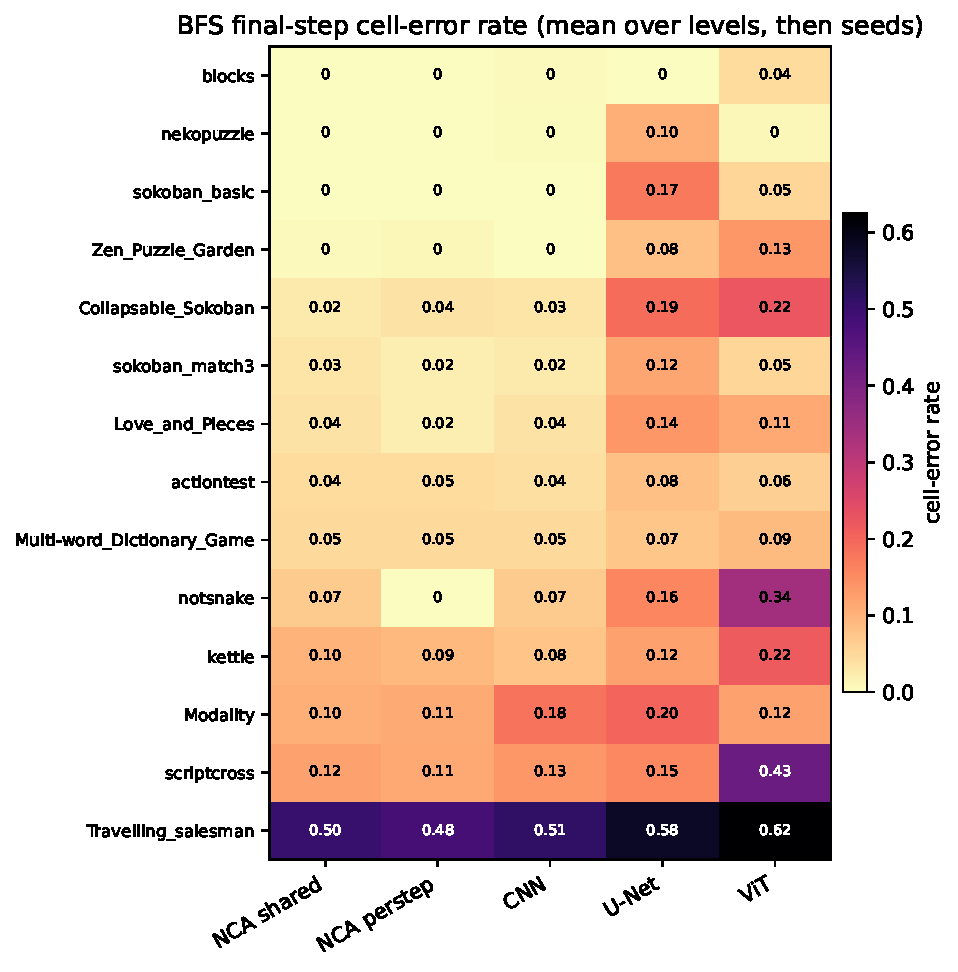
\includegraphics[width=0.95\linewidth]{../figures/baseline_comparison/scaling_14_per_game_heatmap.pdf}
  \caption{\textbf{Per-game BFS final cell-error on
    \textsc{Train-14}.} Rows are games (sorted by NCA-shared error,
    ascending); columns are architectures. Single seed at 20k updates.
    Both NCA variants beat the three non-NCA baselines on the vast
    majority of games; ViT is the only architecture with a
    catastrophic failure on a small game (\textsc{scriptcross}).}
  \label{fig:per-game-heatmap}
\end{figure}

\subsection{Reproducibility}

The codebase, dataset caches, training launchers, and result
aggregators are released alongside the paper. Each run is reproduced
end-to-end by re-running its launcher on the same hardware
(single 24~GB consumer GPU). The full experimental log accompanies
the released code.
% Internal notes (deanonymised paths kept as comments for the
% camera-ready / reproducibility supplement):
%   - Launchers: nca_wm/scripts/run_*.sh
%   - Per-game/per-arch synth grid: nca_wm/scripts/run_per_game_arch_synth_grid.sh
%     summarised via summarize_per_game_arch_grid.py --all_authored_as_heldout
%     and figures via nca_wm/scripts/make_within_game_synth_artifacts.py
%     (logs land in nca_wm/logs_per_game_arch_synth/)
%   - Running-state docs: nca_wm/SCALING_RESULTS.md, nca_wm/ARCHITECTURE_REPORT.md,
%     nca_wm/RUNNING_REPORT.md, project_synth_recipe.md

\section{Per-game $\times$ per-architecture grid}
\label{app:per-game-arch}

To check how architecture choice interacts with game type, we train
one model per (game, architecture-bucket) cell on five games covering
distinct mechanic classes ---
\textsc{Microban} (single-step Sokoban-style box pushing: PuzzleScript's
basic push rule applies force to the cell directly in front of the
player, so a row of two boxes is \emph{not} chained-pushed by a single
action),
\textsc{Heroes\_of\_Sokoban} (multi-bracket character swap and
projectile travel),
\textsc{Bouncers} (non-axis-aligned looping projectile),
\textsc{nekopuzzle} (restricted-orientation movement), and
\textsc{Travelling\_salesman} (multi-bracket all-pairs) --- against
four architecture buckets at $T{=}8$:
(A) pool ON, shared ($n_r{=}T$);
(B) pool ON, per-step ($n_r{=}1$);
(C) no-pool $+$ input-skip, shared;
(D) no-pool $+$ input-skip, per-step.
Each cell is trained on the game's authored level 0 only with the
canonical recipe (\S\ref{sec:experiments}); we evaluate BFS rollout
cell-error on the training level (L0) and on held-out levels
(L1$+$, mean) separately. Training budget is 15k updates per cell,
extended to 50k for \textsc{Travelling\_salesman} after observing
visible loss descent at 15k. Single seed. We also ran the same grid
on \textsc{sokoban\_basic} (a smaller variant of the same Sokoban
dynamics as \textsc{Microban}); the numbers are consistent with the
\textsc{Microban} row and we omit them from the figure to avoid
double-counting the same mechanic.

\begin{figure}[t]
  \centering
  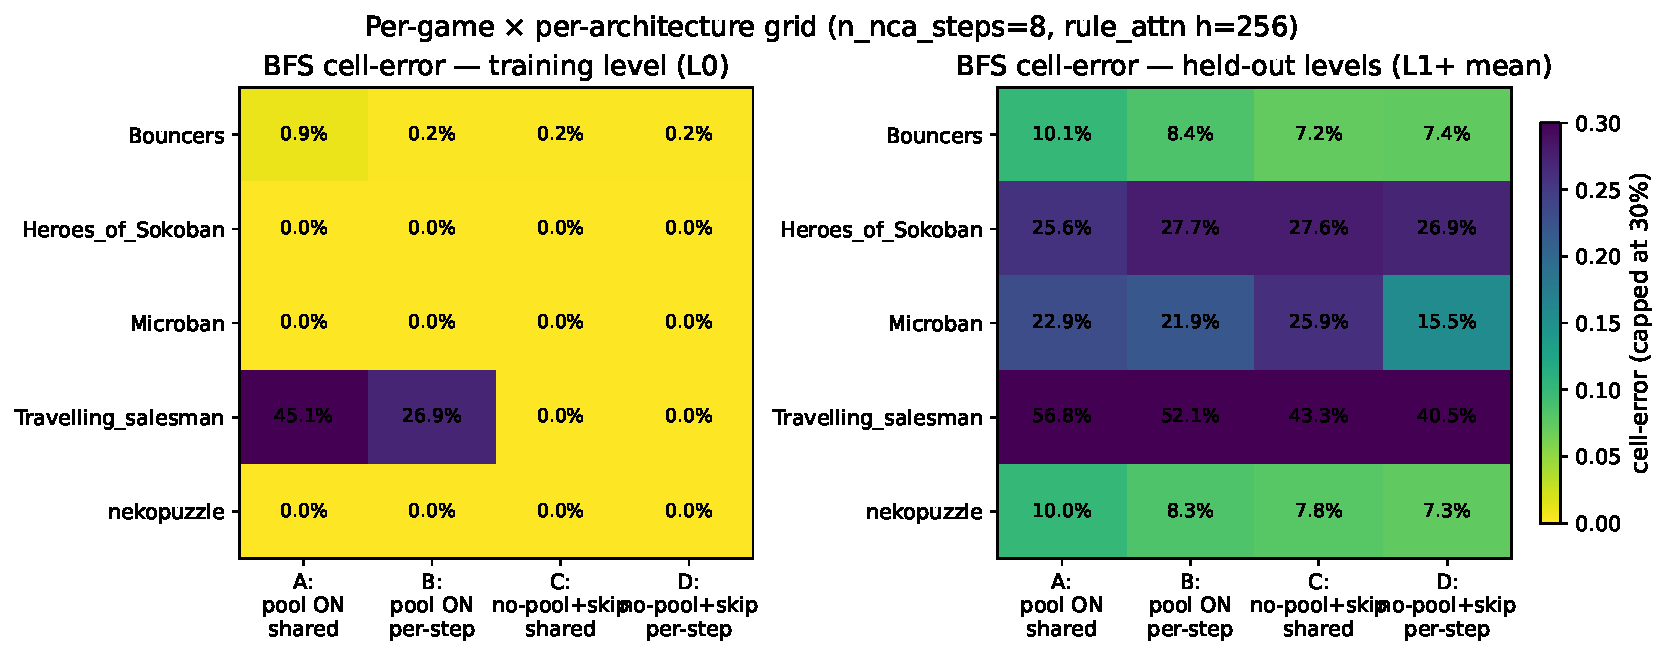
\includegraphics[width=0.98\linewidth]{figures/heatmap_bfs.pdf}
  \caption{\textbf{Per-game $\times$ per-architecture BFS cell-error.}
    Rows: games. Columns: architecture buckets at $T{=}8$. Left panel:
    training-level (L0) cell-error. Right panel: held-out-levels (L1$+$
    mean) cell-error. Cells annotate the percentage. Bucket~D
    (no-pool $+$ input-skip $+$ per-step) wins held-out on five of six
    games. Bucket~A loses dramatically on \textsc{Travelling\_salesman}
    L0 (45.1\%) despite identical train loss to bucket~D (which fits
    L0 to 0\%); see ``F3 sharpened'' below.}
  \label{fig:per-game-arch-heatmap}
\end{figure}

\paragraph{F3 sharpened.}
\S\ref{sec:results-F3} introduced the train-loss-vs-rollout-error
decoupling. The per-game grid pushes the gap to its loudest form yet.
On \textsc{Travelling\_salesman} at 50k updates all four architecture
buckets converge to within $1\%$ of the same train loss
($1.70\times 10^{-3}$ to $1.72\times 10^{-3}$), yet L0 BFS cell-error
splits $0\% / 0\% / 26.9\% / 45.1\%$ across buckets D / C / B / A.
Bucket~A's L0 rollout is in fact \emph{worse} at 50k than at 15k
($45.1\%$ vs.\ $24.0\%$) despite a $68\times$ lower train loss ---
additional optimisation on a per-step minimum that compounds
destructively under autoregressive feedback. Buckets~C and D, which
replace global pool features with input-skip re-injection, converge to
the same train loss with a stable rollout. The pool-ON cells thus
appear to overfit per-step prediction in a way that does not survive
auto-regressive feedback.

\paragraph{Held-out gap and the synth-data prediction.}
Held-out cell-error (right panel of Fig.~\ref{fig:per-game-arch-heatmap})
remains substantial across every cell ($7.3\%$--$56.8\%$). This is the
\emph{within-game} OOD-levels axis --- a complementary, lesser form of
generalization than the OOD-rules / latent-sampling / inverse-fit
claims that the main paper targets. Prior single-game work strongly
predicts that synthetic levels close most of this gap: training
synth-only \textsc{sokoban\_basic} ($w{=}7$) reached $0\%$ cell-error
on the 155 held-out \textsc{Microban} / \textsc{Microban\_I} authored
levels, and multi-grid synth on \textsc{nekopuzzle} closed a
$3$--$8\%$ gap to $0.3\%$ once the synth widths included the authored
aspect ratio. Both signals suggest the right-panel gap here is data
scarcity, not an architectural ceiling.
% Prior-work pointers (deanonymised; kept as comments):
%   - nca_wm/RUNNING_REPORT.md (single-game synth-only Sokoban run)
%   - nca_wm/SCALING_RESULTS.md (multi-grid nekopuzzle synth run)

\paragraph{Synth-only $\to$ all-authored generalization (running).}
\label{app:synth-only}
The within-game-generalization probe replaces each cell's authored
training set with $K{=}128$ synthetic levels generated at the
\emph{smallest-by-area} authored size of the target game and evaluates
on \emph{every} authored level (no L0 / heldout split: all authored
levels are out of distribution to the training set). We anchor on the
smallest authored size because (i) size-up generalization carries
synthetic small-grid training to bigger authored levels (Sokoban
$w{=}7 \to 0\%$ on 155 \textsc{Microban}/\textsc{Microban\_I}
authored levels in prior work) while size-down does not; (ii) using
a single size keeps the per-size data density at $K{=}128$, which
empirically matters: an early multi-grid variant
($K / n_{\text{sizes}}$ per size, $\sim 16$ levels per size for
Microban) plateaued at $\sim 8\%$ BFS heldout while the same recipe
at fixed $K{=}128$ on a single small size reached $0.60\%$ BFS,
$0.02\%$ 1-step. We also tried an auto-bounding-box variant that
picks $\max W \times \max H$ for each game; it failed at $\sim 9\%$
BFS because many authored levels are much smaller than the bounding
box, and the synth distribution missed them. Smallest-by-area (rather
than per-axis $\min W \times \min H$) is used so the chosen size is
an actually-existing authored shape rather than a per-axis composite
(\textsc{Microban}'s per-axis minimum is $6{\times}6$, but no authored
level is $6{\times}6$; smallest-by-area picks $6{\times}7$, which
appears in three authored levels).

The recipe trains on $K{=}128$ synthetic levels at the chosen size for
$30{,}000$ updates with the same four architecture buckets at $T{=}8$,
with synthetic-level generation in \emph{evolve} mode and a small
auxiliary token-decoder loss. To force the GA to spread the $K$-level
budget across the game's rule set rather than collapsing onto a single
easy mechanic, we enable rule-coverage-driven evolution: per-step
rule-firing telemetry biases the fitness to
$\text{BFS-iterations} + 100 \cdot |\text{unique rules fired}|$, and
at the end of evolution we greedily pick the $K$ levels that maximize
the \emph{union} of rules covered (rather than top-$K$ by individual
fitness). For small-rule-set games (e.g.\ Sokoban-class) this is a
no-op; for multi-bracket games (Heroes\_of\_Sokoban,
Travelling\_salesman) it materially changes which $K$ levels enter
training. We also report the iterations-only baseline (no coverage
weighting, no union-greedy selection) as a side-by-side ablation
column in Table~\ref{tab:within-game-synth}. The pre-registered
prediction is in \S\ref{sec:results-within-game}. If pure synth fails
on a game we fall back to seeding from one or a handful of authored
levels alongside synth --- a lesser form of within-game generalization
that still tests few-shot extrapolation.
% Internal pointers (paths kept as comments for the reproducibility
% supplement; they reference deanonymised tooling, so they should not
% appear in the submission body):
%   - Launcher: nca_wm/scripts/run_per_game_arch_synth_grid.sh
%   - Summariser: nca_wm/scripts/summarize_per_game_arch_grid.py
%       --all_authored_as_heldout
%   - Logs land in nca_wm/logs_per_game_arch_synth/
%   - Validated post-1fa557d on Microban, bucket D, 30k updates;
%     see project_synth_recipe.md for full validation history.
%   - Recipe flags:
%     --synthetic_levels 128 --synthetic_w <min_W> --synthetic_h <min_H>
%     --synthetic_fallback_dynamics --synthetic_no_a_count_max 5
%     --synthetic_mode evolve --token_decoder_loss_weight 0.1
%     --synthetic_track_rules_fired --synthetic_rule_coverage_weight 100
%     --synthetic_coverage_select_topk

\papertodo{Fill the synth-only column once the sweep completes:
regenerate the per-game/per-architecture heatmap as a 4-panel figure
(L0 authored vs.\ heldout authored vs.\ synth-only all-authored, with
synth-train-loss as the bonus panel) and update
Table~\ref{tab:within-game-synth}.}

\papertodo{If synth-only beats authored-L0-only on \textsc{Microban}
held-out (Sokoban prior says yes), Heroes\_of\_Sokoban (multi-bracket
char-swap; less certain), and Bouncers (looping projectile; uncertain),
that closes the within-game OOD-levels claim across three distinct
mechanic classes. \textsc{Travelling\_salesman} is the canonical hard
case: if the synth-only run reproduces the F3 sharpening (same train
loss, $40{+}$pp rollout split between buckets) it is the cleanest
demonstration of the per-step-vs-AR decoupling we report, since no
authored memorization remains to confound the comparison.}

\papertodo{\textbf{Extensions.} (i) Add a depth axis $T \in \{4, 16, 32\}$
to test whether bucket A's pool-driven AR-rollout failure shrinks at
larger $T$; (ii) add games covering gravity-chain (\textsc{MazezaM}),
counter / state aggregation (\textsc{Modality}), and length-state
(\textsc{Lime\_Rick}) mechanics; (iii) re-run the existing five cells
with three seeds, since prior work (F8, \S\ref{sec:results-ceiling})
showed per-seed variance can dwarf recipe deltas on similar
single-game multi-grid tasks.}


\end{document}
